\documentclass[11pt%
%,draft%
,aspectratio=169%
]{beamer}
%
\usepackage{fontspec}
\defaultfontfeatures{Ligatures=TeX}
%\setsansfont{Liberation Sans}
\usepackage{polyglossia}
\setdefaultlanguage{german}

%
% Alternative template for talks of the Freie Universität Berlin.
% Created by Leonard R. König, <leonard.koenig@fu-berlin.de> following the
% guidelines on www.fu-berlin.de/cd
%
% (c) Leonard König, CC BY 4.0
%
% This template was written against UTF-8 capable LaTeX engines, specifically
% LuaLaTeX.

% Trying to get rather close to the ppt/odp template:
%  http://www.fu-berlin.de/sites/cd/downloads_container/PowerPoint_Praesentation_Anleitung.pdf

%%% font styles
\setbeamerfont{frametitle}{series=\bfseries}
\setbeamerfont{footline}{series=\bfseries}
\setbeamerfont{headline}{series=\bfseries}
\setbeamerfont{alerted text}{series=\bfseries}
%%%

% colordefs
\definecolor{fu_darkblue}{RGB}{0,51,102}
\definecolor{fu_seablue}{RGB}{0,102,204}
\definecolor{fu_lightblue}{RGB}{204,214,224}
\definecolor{fu_green}{RGB}{153,204,0}
\definecolor{fu_lightgrey}{RGB}{128,128,128}
\definecolor{fu_grey}{RGB}{95,95,95}
%
\definecolor{fu_red}{RGB}{204, 0, 0} % red text (used by \alert)
%%% end colordefs

%%% colors
\setbeamercolor*{title}{fg=fu_darkblue}
\setbeamercolor*{subtitle}{fg=fu_seablue}
\setbeamercolor*{frametitle}{fg=fu_darkblue}
\setbeamercolor*{footline}{fg=fu_grey,bg=fu_lightblue}
\setbeamercolor*{headline}{fg=fu_grey}

\setbeamercolor*{normal text}{fg=black}
\setbeamercolor*{alerted text}{fg=fu_red}
\setbeamercolor*{example text}{fg=fu_green}
\setbeamercolor*{structure}{fg=fu_darkblue}

\setbeamercolor*{block title}{fg=white,bg=black!50}
\setbeamercolor*{block title alerted}{fg=white,bg=black!50}
\setbeamercolor*{block title example}{fg=white,bg=black!50}

\setbeamercolor*{block body}{bg=black!10}
\setbeamercolor*{block body alerted}{bg=black!10}
\setbeamercolor*{block body example}{bg=black!10}

\setbeamercolor{bibliography entry author}{fg=fu_darkblue}

\setbeamercolor{item}{fg=fu_darkblue}
\setbeamercolor{navigation symbols}{fg=fu_lightgrey,bg=fu_grey}
%%% end colors

%%% title page
% Display logo (if exists) and right next to it, put our title + subtitle
\defbeamertemplate*{title page}{fu_titlepage}
{%
	\hskip .3\textheight
	\begin{minipage}[.4\textheight]{\textwidth}
		\begin{minipage}[.4\textheight]{0.25\textwidth}
			\inserttitlegraphic
		\end{minipage}%
		\begin{minipage}[.4\textheight]{0.75\textwidth}
			\begin{beamercolorbox}{title}
				\usebeamerfont{title}\inserttitle\par%
			\end{beamercolorbox}
			\vfill
			\ifx\insertsubtitle
				\@empty%
			\else
				\begin{beamercolorbox}{subtitle}
					\usebeamerfont{subtitle}\insertsubtitle\par
				\end{beamercolorbox}
			\fi
		\end{minipage}
	\end{minipage}%
	\hskip .3\textheight
}
%%% end title page

%%% headline
% display title, author and institute on the left;
% logo on the right.
\newcommand{\headlinetext}
{%
	\inserttitle\\[0.3em]%
	\insertauthor, %
	\insertshortinstitute
}
\newlength{\headlinewidth}
\setlength{\headlinewidth}{\paperwidth}
\addtolength{\headlinewidth}{-2\marginparsep}
\setbeamertemplate{headline}
{%
	\begin{beamercolorbox}[wd=\paperwidth]{headline}%
		\vskip5pt
		{\hspace*{\marginparsep}}%
		\parbox{.5\headlinewidth}
		{%
			\usebeamertemplate{title in head/foot}%
			\headlinetext%
		}%
		\begin{minipage}{.5\headlinewidth}%
			\hfill\usebeamertemplate*{logo}
		\end{minipage}%
		{\hspace*{\marginparsep}}%
	\end{beamercolorbox}%
}
%%% end headline

%%% footline
% title + date on the left, frame number on the right
\newcommand{\footlinetext}
{%
	\usebeamerfont{shorttitle}\insertshorttitle, %
	\usebeamerfont{shortdate}\insertshortdate
}
\setbeamertemplate{footline}
{%
	\begin{beamercolorbox}{footline}
		\vskip2pt
		\hspace{\marginparsep}%
		\footlinetext\hfill%
		\insertframenumber%
		\hspace{\marginparsep}
		\vskip2pt
	\end{beamercolorbox}%
}
%%% end footline

% don't use default templates for sidebars
\setbeamertemplate{sidebar right}{}
\setbeamertemplate{sidebar left}{}
\setbeamertemplate{title page}[fu_titlepage]
%biber stuff
\usepackage[
  backend=biber,
  bibencoding=utf8,
  style=alphabetic,
  %citestyle=authoryear-comp
]{biblatex}
\bibliography{sources.bib}
%
\usepackage{amsmath}
\usepackage{amsfonts}
\usepackage{amssymb}

\usepackage[backend=biber]{biblatex}

%
\usepackage{graphicx}
%tikz stuff
\usepackage{tikz}
\usetikzlibrary{shapes,arrows}

\usepackage{arydshln}
\usepackage{csquotes}
\usetikzlibrary{positioning,shapes,snakes}
\tikzset{main node/.style={circle,fill=blue!20,draw,minimum size=1cm,inner sep=0pt},}
\tikzset{main rectangle/.style={rectangle,fill=blue!20,draw,minimum size=1cm,inner sep=0pt},}
\tikzset{main ellipse/.style={ellipse,fill=blue!20,draw,minimum size=1cm, minimum width=1.5cm,inner sep=0pt},}

\author{Lea Muth \and Benjamin Tröster}
\title[Code-basierte Kryptografie]{Einführung Code-basierte Kryptografie}
\subtitle{Code-basiertes Kryptosystem -- McEliece}
%\pgfdeclareimage{titlegraphic}{pictures/mceliece.png}
%\titlegraphic{\pgfuseimage{titlegraphic}}
\date{\today}
%\subject{}
%
% FU settings
\institute[FU Berlin]{Freie Universität Berlin}
%\pgfdeclareimage[height=0.9cm]{logo}{../res/dwarf_logo}
%\logo{\pgfuseimage{logo}}
%
\begin{document}

\begin{frame}
\titlepage
\end{frame}

\begin{frame}{Fahrplan}
\tableofcontents[hideothersubsections]
\end{frame}

\section*{Zusammmenfassung}
\begin{frame}{Zusammmenfassung}
	\begin{itemize}
		\item McEliece asymmetrisches Public-Key-Kryptosystem -- 1978 nach Robert McEliece \cite{McEliece1978public}
		\item Grundlegende Idee: Führe absichtliche Fehler in die Chiffre ein 
		\item Verwenden eines allgemeinen fehlerkorrigierende Codes
		\begin{itemize}
		    \item Dekodierung i.A. $\mathcal{NP}$-Hart \cite[S. 479]{Schneier2007Applied}, \cite[S. 353ff]{Stinson2018Cryptography}
		    \item Unterklasse an linearen Codes auch in $P$ lösbar $\rightarrow$ Goppa-Codes
		\end{itemize}
		\item Angreifer ohne Goppa-Code kann nur in $\mathcal{P}$, also polynomiell viel rechnen
		\begin{itemize}
		    \item Die Entschlüsselung eines zufälligen linearen Codes ist ein $\mathcal{NP}$-Hartes Problem -> \cite{ljubic2004exact}
		    \item Die Generatormatrix eines Goppa-Codes sieht zufällig aus ->  \cite{6553164} 
		\end{itemize}
	\end{itemize}
\end{frame}

\section{Grundlagen}

\begin{frame}{Fahrplan Grundlagen}
\tableofcontents[currentsection,currentsubsection]
\end{frame}



\subsection{Galoiskörper}
\begin{frame}{Galoiskörper/Galoisfeld}
	\begin{itemize}
		\item Ein Galoiskörper $GF(p)$ , wobei $p$ prim, ist ein endlicher Körper welcher bezüglich '$+$' und '$*$' abgeschlossen ist.\\
		\item Beispiel:\\
		   $GF(2) = \mathbb{F}_{2} = \{0,1\}$: \cite{Kunz1991}\\
		   \begin{align*}
		   Addition: && Multiplikation: \\
		    0+0=0  &&  0*0 = 0 \\
		    0+1=1  &&  0*1 = 0\\
		    1+0=1  &&  1*0 = 0\\
 		    1+1=0  &&  1*1 = 1\\
		    \end{align*}
	\end{itemize}
\end{frame}
 
\subsection{Hamming Gewicht und Distanz}
\begin{frame}{Hamming Gewicht}
	\begin{itemize}
		\item Das Hamming Gewicht $w(\cdot)$ eines Vektors $x$ mit Länge $n$ ist definiert als:
		\begin{align*}
		w(x):= \sum_{i=1}^n w(x_i) \qquad mit \qquad w(x_i) =
		\begin{cases}
		w(x_i) = 1: x_i \neq 0 \\
		& \cr w(x_i) =0 : x_i = 0
		\end{cases}
		\end{align*}
     	\item Beispiel:
     		\begin{align*}	
     		    w(\underline{1}00\underline{1})  = 2\\
     			w(0\underline{1}\underline{1}\underline{1})  = 3
     		\end{align*}
	\end{itemize}
\end{frame}


\begin{frame}{Hamming Distanz}
	\begin{itemize}
		\item Hamming Distanz $D(\cdot, \cdot)$ zwischen zwei validen Codewörten $c$ und $c'$ ist definiert als: 
		\[D(c,c'):=|\{i \in \{1,\ldots,n\}| c_{i}\neq c'_{i} \}|
		\]
		\item Beispiel:
			\begin{align*}
		    	D(\underline{0}\underline{0}\underline{0},\underline{1}\underline{1}\underline{1}) = 3 \\
		        D(0011\underline{0},0011\underline{1}) = 1 \\
		        D(\vec{c},0000) = w(\vec{c})
		    \end{align*}
	\end{itemize}
\end{frame}

\begin{frame}{Minimale Hamming Distanz}
	\begin{itemize}
		\item Die minimale Hamming Distanz d ist die kleinste Hamming Distanz zwischen zwei beliebigen gültigen Codewörten. 
		\[d=\min_{c\neq c'}D(c,c')\]
		\item Beispiel:~ $d=3$ \\
\begin{tabular}{cc} 
 \hspace*{-.3cm} 
 \parbox{0.55\linewidth}{
	\begin{table}[]
\begin{tabular}{c}
\hline
Codewort \\ \hline
000      \\
111     
\end{tabular}
\end{table}

} 
& \begin{tabular}{c}
 \begin{tabular}{c}
    \centering
        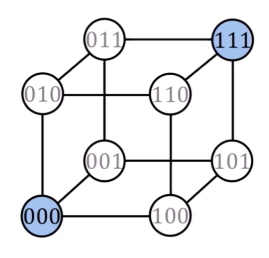
\includegraphics[scale=0.60]{pictures/d_gleich_3_bsp}
\end{tabular}
\end{tabular}\\
\end{tabular}
	\end{itemize}
	\end{frame}
	
\begin{frame}{Minimale Hamming Distanz}
	\begin{itemize}
		\item Beispiel:~ $d=2$
	\end{itemize}
\begin{tabular}{cc} 
 \hspace*{-.3cm} 
 \parbox{0.35\linewidth}{
      \begin{table}[]
      \begin{tabular}{c}
      \hline
      Codewort \\ \hline
      0000      \\
      0011      \\
      1100      \\
      1111      
      \end{tabular}
      \end{table}
} 
& \begin{tabular}{c}
 \begin{tabular}{c}
        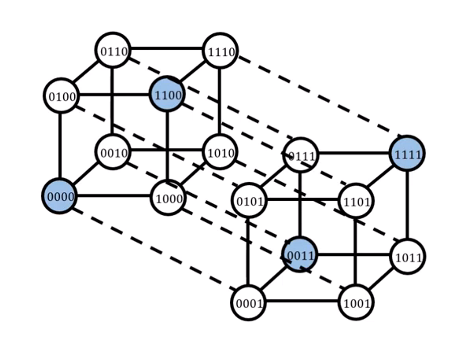
\includegraphics[scale=0.60]{pictures/d_gleich_2_bsp}
\end{tabular}
\end{tabular}\\
\end{tabular}
\end{frame}

\begin{frame}{Minimale Hamming Distanz}
	\begin{itemize}
		\item Beispiel:~ $d=1$ 
	\end{itemize}
\begin{tabular}{cc} 
 \hspace*{-.3cm} 
 \parbox{0.35\linewidth}{
      \begin{table}[]
      \begin{tabular}{c}
      \hline
      Codewort \\ \hline
      0000      \\
      0001      \\
      1110      \\
      1111      
      \end{tabular}
      \end{table}
} 
& \begin{tabular}{c}
 \begin{tabular}{c}
        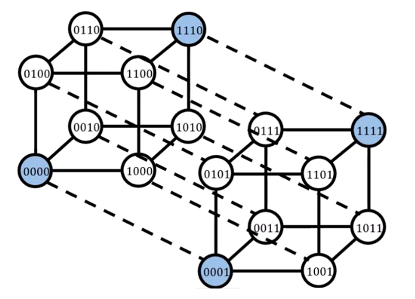
\includegraphics[scale=0.60]{pictures/d_gleich_1_und_3_bsp.png}
\end{tabular}
\end{tabular}\\
\end{tabular}
\end{frame}

\begin{frame}{Hamming Code Projektion}
\begin{tabular}{cc} 
 \hspace*{-.3cm} 
 \parbox{0.4\linewidth}{
	\begin{itemize}
	\item Ein $(7,4)$ Hamming-Code ohne mgl. Fehlerkorretur, da $d=1$
	\item Projektion von $4d \to 7d$
		\begin{itemize}
		    \item D.h. 4 Bit Nachricht $abcd$ auf 7 Bit Code-Wort $abcd~xzy$ abgebildet
		\end{itemize}
		\item Bsp. $abcd \to abcd~xyz$ 
		\begin{align*}
		    x&= a \oplus b \oplus d\\
		    y&= a \oplus c \oplus d\\
		    z&= b \oplus c \oplus d
		\end{align*}
    \end{itemize}
} 
& \begin{tabular}{c}
 \begin{tabular}{c}
        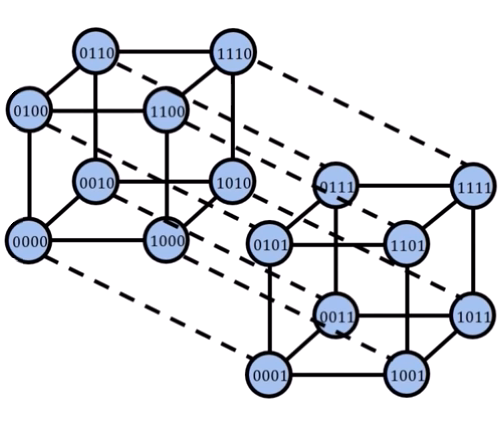
\includegraphics[scale=0.60]{pictures/hamming_7_4_d_gleich_1.png}
\end{tabular}
\end{tabular}\\
\end{tabular}
\end{frame}


\begin{frame}{Hamming Code}
	\begin{itemize}
		\item Beispiel:
		\begin{align*}
		  abcd \to abcd~xyz && x&= a \oplus b \oplus d\\
		  1001 \to 1001001 && y&= a \oplus c \oplus d\\
		  0010 \to 0010011 && z&= b \oplus c \oplus d
		\end{align*}

	\end{itemize}
\end{frame}






\begin{frame}{Hamming Code}
	\begin{itemize}
		\item Check-Bits $xyz$ können folgende Check-Bit-Status haben (Syndrome s)
		\begin{table}[]
        \begin{tabular}{l|lll}
        \textbf{x y z} & \textbf{Error-State} & \textbf{a b c d} & \textbf{x y z}\\ \hline
        \checkmark \checkmark \checkmark& no error & \checkmark\checkmark\checkmark\checkmark & \checkmark\checkmark\checkmark \\
        $\times$ \checkmark \checkmark& x is wrong & \checkmark\checkmark\checkmark\checkmark & $\times$\checkmark\checkmark \\
        \checkmark  $\times$  \checkmark& y is wrong & \checkmark\checkmark\checkmark\checkmark &\checkmark $\times$\checkmark \\
        \checkmark \checkmark  $\times$ & z is wrong & \checkmark\checkmark\checkmark\checkmark & \checkmark\checkmark $\times$ \\ \hdashline
        $\times$ $\times$ \checkmark& a is wrong & $\times$\checkmark\checkmark\checkmark & \checkmark\checkmark\checkmark \\
        $\times$ \checkmark$\times$ &b is wrong & $\times$\checkmark\checkmark\checkmark & \checkmark\checkmark\checkmark \\
        \checkmark$\times$ $\times$ & c is wrong & \checkmark\checkmark$\times$\checkmark & \checkmark\checkmark\checkmark \\
        $\times$ $\times$ $\times$ & d is wrong & \checkmark\checkmark\checkmark $\times$ & \checkmark\checkmark\checkmark \\
        \end{tabular}
        \end{table}
	\end{itemize}
\end{frame}


\begin{frame}{Hamming Code}
	\begin{itemize}
        \item Aus den Spalten können die Gleichungen wie folgt abgeleitet werden:
        \begin{table}[]
\begin{tabular}{l|l}
& \textbf{x y z} \\ \hline
a is wrong & $\times$ $\times$\checkmark \\
b is wrong & $\times$\checkmark $\times$ \\
c is wrong & \checkmark $\times$ $\times$ \\
d is wrong &  $\times$ $\times$ $\times$ \\
\end{tabular}
\item
    \begin{align*}
		    x&= a \oplus b \oplus d\\
		    y&= a \oplus c \oplus d\\
		    z&= b \oplus c \oplus d
		\end{align*}
\end{table}
	\end{itemize}
\end{frame}

\begin{frame}{Hamming Code}
	\begin{itemize}
		\item Beispiel: (Fehlerkorrektur)
		\begin{align*}
		  abcd~xyz && x&= a \oplus b \oplus d\\
		  1001~010 && y&= a \oplus c \oplus d\\
		   && z&= b \oplus c \oplus d
		\end{align*}

	\end{itemize}
\end{frame}



\subsection{Generatormatrix}
\begin{frame}{Generatormatrix I}
	\begin{itemize}
		\item Ein linearer binärer $(n,k,d)$-Code $C$ kann durch die Generatormatrix $G$ wie folgt charakterisiert werden:
			\[C =\{c \in GF(2^n), m \in GF(2^k): c=m\cdot G\} \] 
			
        \begin{itemize}
            \item $n$ Länge des Codeworts
             \tikz[remember picture] \node[coordinate,yshift=0.5em] (n1) {}; 
            \item $k$ Nachrichtenlänge
            \tikz[remember picture] \node[coordinate] (n2) {};
            \item $d$ minimale Distanz
            \tikz[remember picture] \node[coordinate] (n3) {};
        \end{itemize}
			\item Beispiel:\\ 
			\begin{itemize}
		 \item$G=\begin{pmatrix} 1 & 0 & 0 & 0 & 1 & 1 & 0  \\ 0 & 1 & 0 & 0 & 1 & 0 & 1  \\ 0 & 0 & 1 & 0 & 0 & 1 & 1 \\0 & 0 & 0 & 1 & 1 & 1 & 1 \end{pmatrix}$
		  (Hamming$(7,4)$-Code mit der Generatormatrix G)
		 	\end{itemize}	
	\end{itemize}
\end{frame}

\begin{frame}{Generatormatrix II}
	\begin{itemize}
		\item Beispiel:\\
		Nachricht $m$ wird mittels der Generatormatrix $G$ in das zugehörige in das jeweilige Codewort $c$ transformiert und es gilt $m \cdot G=c$:\\
		~\\
        $$\begin{pmatrix} a & b & c & d\end{pmatrix} \cdot \begin{pmatrix} 1 & 0 & 0 & 0 & 1 & 1 & 0  \\ 0 & 1 & 0 & 0 & 1 & 0 & 1  \\ 0 & 0 & 1 & 0 & 0 & 1 & 1 \\0 & 0 & 0 & 1 & 1 & 1 & 1 \end{pmatrix} = \begin{pmatrix} a&b&c&d &&x&y&z\end{pmatrix}$$

	\end{itemize}
\end{frame}


\subsection{Parity-Check-Matrix}
\begin{frame}{Parity-Check-Matrix / Prüfmatrix}
    \begin{itemize}
        \item Ein linearer binärer $(n,k,d)$-Code $C$ kann durch die Prüfmatrix $H$ wie folgt charakterisiert werden:
			\[C =\{c \in GF(2^n) : H\vec{c}^T =\vec{0}\} \] 
 
        \item Bsp.: Hamming-Code $(7,4)$ mit Parity-Check-Bit-Gleichungen $abcd~xyz$
        \begin{align*}
		    a \oplus b \oplus d &= x\\
		    a \oplus c \oplus d &= y\\
		    b \oplus c \oplus d &= z
		\end{align*}

    \end{itemize}
\end{frame}

\begin{frame}{Parity-Check-Matrix / Prüfmatrix}   
\begin{itemize}
	\item Durch umformen erhalten wir ($\oplus \equiv -$):
		\begin{align*}
		    a \oplus b \oplus 0c \oplus d \oplus x \oplus 0y \oplus 0z &= 0\\
		    a \oplus 0b \oplus c \oplus d \oplus 0x \oplus  y \oplus 0z &= 0\\
		    0a \oplus b \oplus c \oplus d \oplus 0x \oplus 0y \oplus z &= 0
		\end{align*}
	

		\item LGS kann als Matrix geschrieben werden, alle validen Codeworte erfüllen dies
		\begin{align*}
		    \begin{pmatrix}
		            1 & 1 & 0 & 1 & 1 & 0 & 0 \\
		            1 & 0 & 1 & 1 & 0 & 1 & 0 \\
		            0 & 1 & 1 & 1 & 0 & 0 & 1 
		    \end{pmatrix} 
		    \cdot 
		    \begin{pmatrix}
		            a\\b\\c\\d\\x\\y\\z
		    \end{pmatrix}^T
		    =
		    \begin{pmatrix}
		          0\\0\\0  
		    \end{pmatrix}
		\end{align*}
    \end{itemize}
\end{frame}

\begin{frame}{Parity-Check-Matrix Beispiel}
    \begin{itemize}
        \item Ist $1101100$ ein valides Codewort?
        \item Für valide Codewörter gilt: $H\cdot \Vec{c}^T = \Vec{0}$ 
        \item Wende $H$ auf $\Vec{c}^T$ an:
        \begin{align*}
            H \cdot \vec{c}^T =
             \begin{pmatrix}
		            1 & 1 & 0 & 1 & 1 & 0 & 0 \\
		            1 & 0 & 1 & 1 & 0 & 1 & 0 \\
		            0 & 1 & 1 & 1 & 0 & 0 & 1 
		    \end{pmatrix} \cdot
		    \begin{pmatrix}
                1\\1\\0\\1\\1\\1\\0\\0 
		    \end{pmatrix}^T =
		    \begin{pmatrix}
		       0\\0\\0
		    \end{pmatrix}
        \end{align*}

    \end{itemize}
\end{frame}

\begin{frame}{Parity-Check-Matrix Beispiel}
    \begin{itemize}
       \item Durch addieren eines Fehlers $H (\Vec{c} + \Vec{e})^T = H \cdot \Vec{c}^T + H \cdot \Vec{e}^T = H \cdot\Vec{e}^T$
        \begin{align*}
            H \cdot \vec{c}^T =
             \begin{pmatrix}
		            1 & 1 & 0 & 1 & 1 & 0 & 0 \\
		            1 & 0 & 1 & 1 & 0 & 1 & 0 \\
		            0 & 1 & 1 & 1 & 0 & 0 & 1 
		    \end{pmatrix} \cdot
		    \begin{pmatrix}
                1\\1\\0\\1\\1\\1\\0\\0 
		    \end{pmatrix}^T\cdot
		    \begin{pmatrix}
                0\\1\\0\\0\\0\\0\\0\\0 
		    \end{pmatrix}^T =
		    \begin{pmatrix}
		       0\\0\\0
		    \end{pmatrix}^T
		    +	    \begin{pmatrix}
		       1\\0\\1
		    \end{pmatrix}^T =  \begin{pmatrix}
		       1\\0\\1
		    \end{pmatrix}^T
        \end{align*}
    \end{itemize}

\end{frame}

\begin{frame}{Recap / Idee der fehlerkorrigierenden Codes}
 \begin{tabular}{cc} 
 \hspace*{-.3cm} 
 \parbox{0.35\linewidth}{
	\begin{itemize}
        \item Gültige Codewörter helfen nicht bei der Fehlerkorrektur
        \item Ungültige helfen, da wir diese \enquote{auseinander} ziehen können
    \end{itemize}
} 
& \begin{tabular}{l}
 \begin{tabular}{c}
    \begin{tikzpicture}
    \node[main node] (1) {food};
    \node[main rectangle] (2) [left = of 1]  {f\underline{r}od};
    \node[main ellipse] (3) [right = of 1] {good};
    \node[main ellipse] (4) [above right = of 1] {wood};
    \node[main rectangle] (5) [below right = of 1] {\underline{e}ood};
    \node[main rectangle] (6) [below = of 1] {fo\underline{q}d};
    \node[main ellipse] (7) [below left = of 1] {fool};
    \node[main ellipse] (8) [above left = of 1] {foot};
    \node[main ellipse] (9) [above = of 1] {foox};
    
    \path[-] (1) edge node {} (2);
    \path[-] (1) edge node {} (3);
    \path[-] (1) edge node {} (4);
    \path[-] (1) edge node {} (5);
    \path[-] (1) edge node {} (6);
    \path[-] (1) edge node {} (7);
    \path[-] (1) edge node {} (8);
    \path[-] (1) edge node {} (9);
    \end{tikzpicture}
\end{tabular}
\end{tabular}\\
\end{tabular}
\end{frame}




\begin{frame}{Recap / Idee der fehlerkorrigierenden Codes}
 \begin{tabular}{cc} 
 \hspace*{-.3cm} 
 \parbox{0.65\linewidth}{
	\begin{itemize}
        \item Generatormatrix $G = [1,1,1]$ transformiert $1$-Bit Nachrichten in $3$-Bit Codeworte
        \item Fehler können angeordnet werden, durch das Füllen der Lücken mit ungültigen Codeworten werden Fehler zuordenbar und  korrigierbar
         \item Beispiel: \\
         $0\cdot[111] \to [0,0,0]$ und $1\cdot[1,1,1] \to [0,0,0]$ 
    \end{itemize}
} 
& \begin{tabular}{c}
 \begin{tabular}{c}
        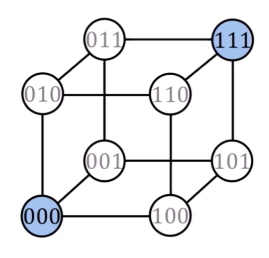
\includegraphics[scale=0.7]{pictures/d_gleich_3_bsp}
\end{tabular}
\end{tabular}\\
\end{tabular}
\end{frame}

\begin{frame}{Beispiel Hamming(7,4)-Code}
\begin{figure}
    \centering
    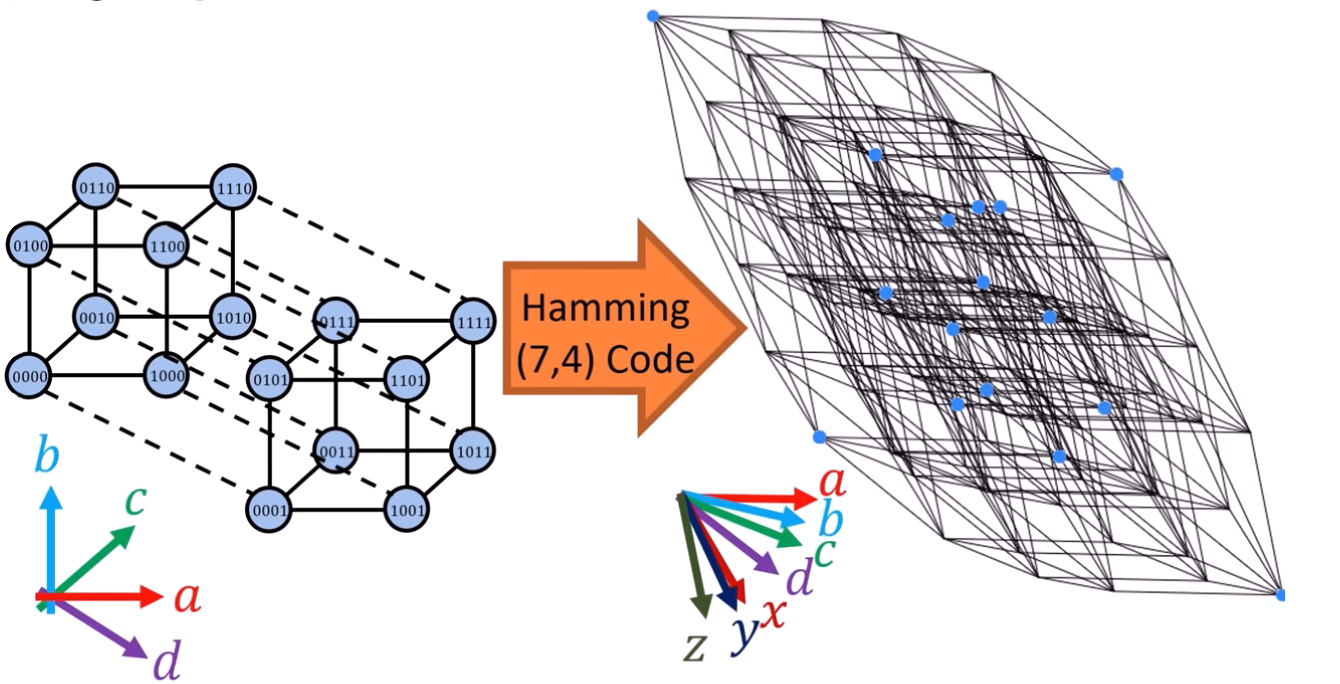
\includegraphics[scale=0.35]{pictures/hamming_7_4_bsp.png}
    \label{fig:my_label}
\end{figure}
\end{frame}

\subsection{Lineare Codes}
\begin{frame}{Lineare Codes}
	\begin{itemize}
		\item \textbf{Defintion:} Ein binärer $(n,k,d)$-Code ist linear, die $\oplus$-Summe zweier beliebiger gültiger Codeworte $c$ und $c'$ wiederum ein gültiges Codewort ergibt:
			\[\forall c,c' \in C \colon c\oplus c' \in C \]
			\begin{itemize}	
		     \item Beispiel: $(0,1,1)+(0,1,1)=(0,0,0)$
	    	\end{itemize}
		\item Bei gegebener Hamming Distanz $d$ wird der Code C auch $(n,k,d)$-Code genannt

	\end{itemize}
\end{frame}



\subsection{Zyklischer Code}
\begin{frame}{Zyklischer Code}
\begin{itemize}
	\item \textbf{Definition:} Ein binärer $(n,k,d)$-Code heißt zyklisch, wenn jede zyklische Verschiebung (Shift) eines gültiges Codewortes $c$ wiederum ein gültiges Codewort ergibt:
			\[\forall ~ c=(c_1,c_2,\dots,c_n) \in C \implies c'=(c_n,c_1,c_2,\dots,c_{n-1}) \in C \]
			\begin{itemize}	
		     \item Beispiel: $(10100) \in C \implies (01010) \in C$
	    	\end{itemize}
	\end{itemize}
\end{frame}

\subsection{Zyklischer linearer Code}
\begin{frame}{Zyklischer linearer Code}
\begin{itemize}
	\item \textbf{Defintion:} Ein binärer $(n,k,d)$-Code ist linear und zyklisch wenn:
			\begin{itemize}	
		     \item Die $\oplus$-Summe zweier beliebiger Codeworte $c$ und $c'$ wiederum ein gültiges Codewort ergibt:
			\[\forall c,c' \in C \colon c\oplus c' \in C \]

	    \item Jede zyklische Verschiebung eines Codeworte $c$ wiederum ein gültiges Codewort ergibt:
			\[\forall ~ c=(c_0,c_1,\dots,c_{n_1}) \in C \implies c'=(c_{n_1},c_0,c_1,\dots,c_{n_2}) \in C \]

	    	\end{itemize}
\end{itemize}
 \end{frame}
 
\begin{frame}{Zyklischer linearer Code}
		\begin{itemize}	
		\item Beispiel:\\
		Gegeben ein Generatorcodewort (100100):
	    	\begin{itemize}	
		     \item Mehrfaches Verschieben bis hin zum ursprünglichen Codewort 
		     \[(100100) \implies (010010) \implies (001001)\implies (100100)\]
	    	\end{itemize}

	    	\end{itemize}
 
\end{frame}

\begin{frame}{Zyklischer linearer Code}
		\begin{itemize}	
		\item Beispiel:\\
		Gegeben ein Generatorcodewort $c_{gen}$ (100100):
	    	\begin{itemize}	
		     \item Addieren um die restlichen Codeworte zu erhalten:
		     \begin{align*}
		        (100100) + (100100) &= (000000)\\
		     (100100) + (010010) &= (110110)\\
		    (100100) + (001001) &= (101101)\\
		     (010010) + (101101) &= (111111)
		       \end{align*}
	    	\end{itemize}
	    	\end{itemize}
 
\end{frame}

\begin{frame}{Zyklischer linearer Code in polynomialer Darstellung}
	\begin{itemize}	
		\item 	Die Zeichen eines Codewortes $c$ lassen sich als Koeffizienten eines Polynomes $c(x)$ betrachten:
		\[\forall  c=(c_0,c_1,\dots,c_{n_1}) \iff c(x) = c_0 + c_1x + \dots + c_{n_1}\]
	  \item Das Polynom des Generatorcodewortes ist das Generatorpolynom\\
	    	\begin{itemize}	
		     \item Beispiel:
		     \begin{align*}
		         (1011) &= \underline{1}\cdot X^0+= \underline{0}\cdot X^1+= \underline{1}\cdot X^1+= \underline{1}\cdot X^3
		     \end{align*}
		   	\end{itemize}
    \end{itemize}
\end{frame}

\subsection{Generatorpolynom}
\begin{frame}{Generatorpolynom}
	\begin{itemize}	
	\item \textbf{Defintion:} Ein von null verschiedenes Polynom $g$ minimalen Grades eines zyklischen Codes heißt Generatorpolynom.
	\item  Ein zyklischer Code der Länge $n$ mit einem Generatorpolynom $g$ des Grades $r$ hat einen Coderaum der Dimension $r=n-k$ und codiert somit $r$ -viele Bits pro Codewort.
	
	\end{itemize}
\end{frame}
 
 
\subsection{Generatorpolynom}
\begin{frame}{Generatorpolynom}
\begin{tabular}{cccc} 
 \hspace*{-.3cm} 
 \parbox{0.55\linewidth}{
\begin{table}[]
\begin{tabular}{ll}
\hline
\multicolumn{1}{l}{Nachricht} & \multicolumn{1}{l}{Codewortpolynomial} \\ \hline
0                              &    0                                   \\
1                              &     $x^3+1$                                    \\
x                              &       $x^4+x$                                     \\
$x+1$                            &  $x^4+x^3+x+1$                                          \\
$x^2$                         &     $x^5+x^2$                                       \\
$x^2+1$                         &     $x^5+x^3+x^2+1$                                       \\
$x^2+x$                         &      $x^5+x^4+x^2+x$                                       \\
$x^2+x+1$                         &     $x^5+x^4+x^3+x^2+x+1$                                        
\end{tabular}
\end{table}
} 
& \begin{tabular}{c}
 \begin{tabular}{c}
        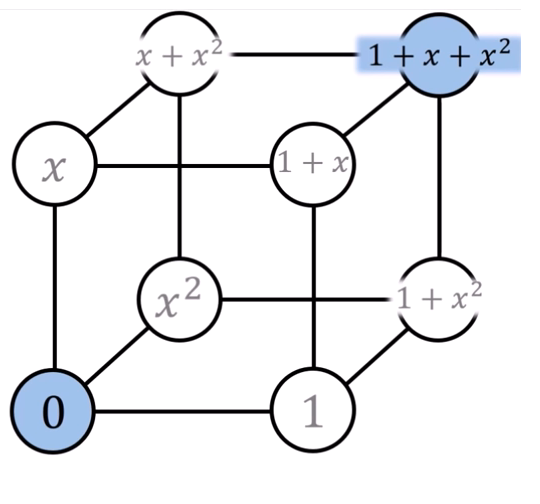
\includegraphics[scale=0.40]{pictures/genpolynom_3_d.png}
\end{tabular}
\end{tabular}\\
\end{tabular}
\end{frame}

\begin{frame}{Recap Generatormatrix / Generatorpolynom}
\begin{tabular}{cccc} 
 \hspace*{-.3cm} 
 \parbox{0.45\linewidth}{
    \begin{table}[]
    \begin{tabular}{cc}
    \hline
    Nachricht & Codewort \\ \hline
    0         & 00       \\
    1         & 11      
    \end{tabular}
    \end{table}
} 
& \begin{tabular}{c}
 \begin{tabular}{c}
        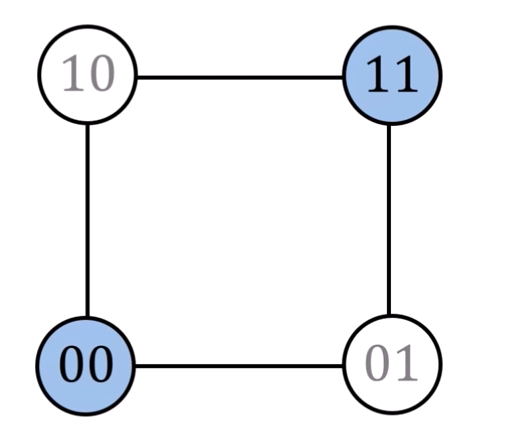
\includegraphics[scale=0.225]{pictures/gen_matrix_polynom_vergleich_2_d_matrix.png}
\end{tabular}
\end{tabular}\\
\parbox{0.45\linewidth}{
    \begin{table}[]
    \begin{tabular}{cc}
    \hline
    Nachricht & Codewort \\ \hline
    0         & 0       \\
    1         & $1+x$      
    \end{tabular}
    \end{table}
} &\begin{tabular}{c}
 \begin{tabular}{c}
        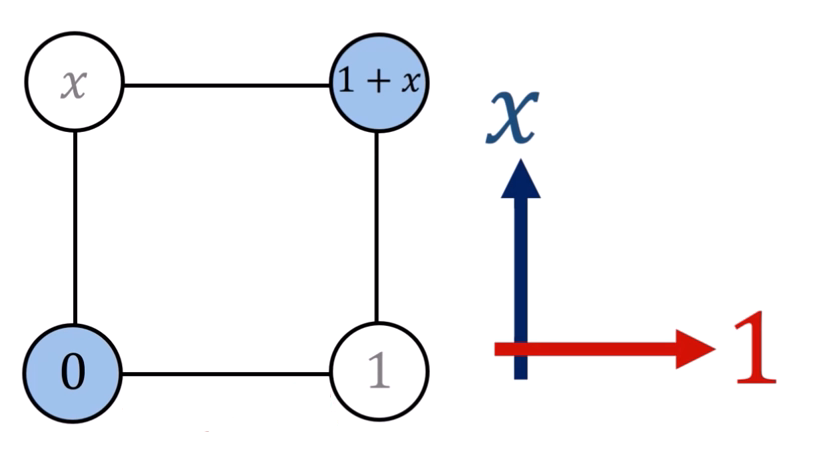
\includegraphics[scale=0.225]{pictures/gen_matrix_polynom_vergleich_2_d_poylnom.png}
\end{tabular}
\end{tabular}\\
\end{tabular}
\end{frame}

\begin{frame}{Recap Generatormatrix / Generatorpolynom}
\begin{tabular}{cccc} 
 \hspace*{-.3cm} 
 \parbox{0.45\linewidth}{
    \begin{table}[]
    \begin{tabular}{cc}
    \hline
    Nachricht & Codewort \\ \hline
    0         & 000       \\
    1         & 111      
    \end{tabular}
    \end{table}
} 
& \begin{tabular}{c}
 \begin{tabular}{c}
        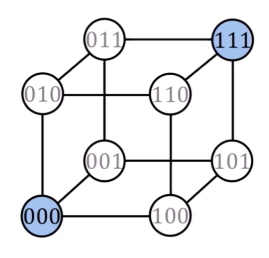
\includegraphics[scale=0.50]{pictures/d_gleich_3_bsp.png}
\end{tabular}
\end{tabular}\\
\parbox{0.45\linewidth}{
    \begin{table}[]
    \begin{tabular}{cc}
    \hline
    Nachricht & Codewort \\ \hline
    0         & 0       \\
    1         & $1+x+x^2$      
    \end{tabular}
    \end{table}
} &\begin{tabular}{c}
 \begin{tabular}{c}
        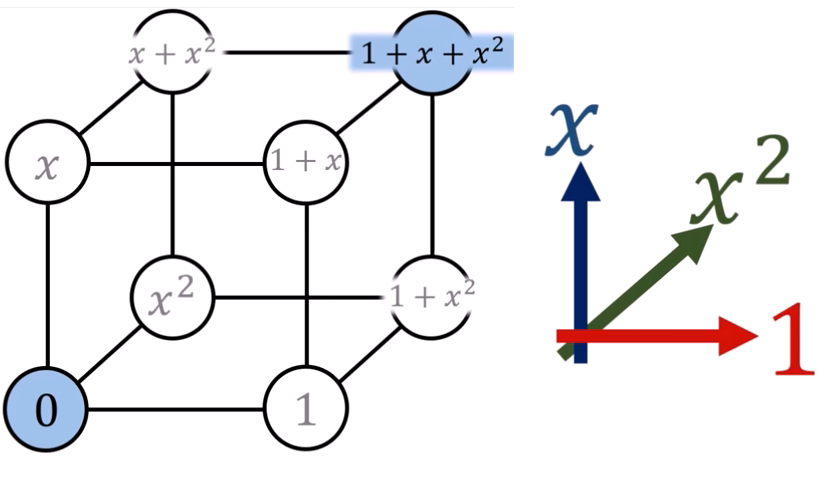
\includegraphics[scale=0.25]{pictures/gen_matrix_polynom_vergleich_3_d_poylnom.png}
\end{tabular}
\end{tabular}\\
\end{tabular}
\end{frame}


\begin{frame}{Goppa-Code}
	\begin{itemize}
		\item Ein binärer Goppa-Code ist ein linearer zyklischer $(n,k,d)$-Code, der durch ein Generatorpolynom $g$ definiert ist und $\lfloor \frac{d-1}{2} \rfloor$ Fehler korrigieren kann. 

	
  \end{itemize}
\end{frame}

\subsection{McElice Kodierungsproblem}
\begin{frame}{McElice Kodierungsproblem}
    \begin{itemize}
        \item McElice basiert auf klassischen Dekodierungsproblemen \cite{berlekamp1978inherent}
        \item Sei $C$ ein linearer $(n,k)$ Code über $\mathbb{F}$ und $y \in C$ das empfangene Codewort
        \item Somit ist $s = y \cdot H$ Syndrom des empfangenen Worts, wobei $H$ die Parity-Check-Matrix ist
        \item Die beste Abschätzung der empfangen Nachricht des Codeworts ist $x= y + z_0$ ($z$ Fehlervektor), wobei $z_0$ minimal bzgl. der Gleichung $s=z \cdot H$ ist
        \item Problem: finde $x \in C$ mit minimaler Distanz zwischen $y,x$ 
        \item Im Mittel muss jedoch die gesamte Lösungsmenge für $s=y \cdot H$ durchsucht werden, um die minimale Distanz zu finden
        \begin{itemize}
            \item Größe des Lösungsraums ist jedoch $2^k$
        \end{itemize}
        \item Ein Algorithmus $\mathcal{A}$ mit gegebener Matrix $H$ und Vektor $s$ soll die Lösung der minimale Gewichtung für $y \cdot H = s$ finden, kann für die Eingabe nur eine Exponentialfunktion sein.
    \end{itemize}
\end{frame}

\subsection{McElice Kodierungsproblem}
\begin{frame}{McElice Kodierungsproblem}
    \begin{itemize}
        \item Beweis der $\mathcal{NP}$-Härte in \cite{berlekamp1978inherent} via Reduktionsbeweis der Entschediugngsprobleme
        \begin{itemize}
            \item Coset-Weight
            \item Subspace-Weight
        \end{itemize}
    \end{itemize}
\end{frame}


\section{McEliece -- Code-basierte Kryptografie}

\begin{frame}{Fahrplan Code-basierte Kryptografie}
\tableofcontents[currentsection,currentsubsection]
\end{frame}


\subsection{McEliece-Kryptosystem}

\begin{frame}{Grundlegende Idee McEliece Kryptosystem}
	\begin{itemize}
		\item Transformiere Klartext $m$ (Message) mithilfe einer Generator-Matrix in allgemeinen Goppa-Code
		\item Multiplikation mit randomisierten Matrizen führt zu allgemeinem linearen Code
		\begin{itemize}
		    \item Gist: Reihe von Matrix-Multiplikationen ist Verschlüsselung
		\end{itemize}
		\item Retransformation ohne Matrizen in Goppa-Code ist problemtisch: $\mathcal{NP}$-Hart \cite{Stinson2018Cryptography}
        \item Öffentlicher Schlüssel:
        \begin{itemize}
            \item Beinhaltet Generator-Matrix zur Umwandlung in allg. linearen Code
            \item Zusätzlich: Anzahl der maximal einbaubaren Fehler in der Chiffre $c$
            \item Fehler sind also die Anzahl der Bits, die invertiert werden sollen
        \end{itemize}
	    \item Privater Schlüssel: Umwandlung des allgemeinen, linearen Codes in Goppa-Code
	    \begin{itemize}
	        \item Für performante Retransformation
	        \item Und Fehlerkorrektur
	    \end{itemize}
	\end{itemize}
\end{frame}
 

\subsection{Parameter Definitionen}
\begin{frame}{Parameter Definitionen}
    \begin{itemize}
        \item Systemparameter $m$ gibt die Blockgröße an, für zu verschlüsselnde Nachricht
        \item $C$ sei ein binärer $(n,k)$ Goppa-Code mit $t$ effizient korrigierbaren Fehlern
        \item $t$ gibt die maximale Anz. eff. korrigierbarer Fehler durch Goppa-Code $C$ \footnote{McEliece fixiert $t=50$, als Maximalwert \cite{McEliece1978public}}
        \item Daraus ergeben sich:
        \begin{itemize}
            \item Blocklänge Chiffretext: $n = 2^m$
            \item Nachricht Blocklänge $k = n - m \cdot t$
            \item Minimale Hamming-Distanz $d$ des Codes $C$: $d = 2 \cdot t + 1$
        \end{itemize}
    \end{itemize}   
\end{frame}

\subsection{McEliece Algorithmus}
\begin{frame}{McEliece als CPA-Sicheres kryptografisches Shema}
    \begin{itemize}
        \item Das \emph{McEliece}-Kryptosystem $\Pi := (Gen, Enc, Dec)$
        \item Wobei:
        \begin{itemize}
            \item $Gen$ Schlüsselerzeugung
            \item $Enc$ Verschlüsselung
            \item $Dec$ Entschlüsselung
        \end{itemize}
        \item Korrekheit: Es muss gelten
        $$
            m = Dec_{priv}(c) = Dec_{priv} (Enc_{pub}(m))
        $$
    \end{itemize}
\end{frame}

\subsection{Schlüsselerzeugung $Gen$}
\begin{frame}{Schlüsselerzeugung $Gen$}
\begin{itemize}
    \item Erzeuge Generator-Matrix $G^{k \times n}$  für Goppa-Code $C$
    \begin{itemize}
        \item Matrix aus der binärer Klartext mit Länge $k$ die Chiffre der Länge $n$ berechnet werden kann
    \end{itemize}
    \item Erzeuge zufällige, binäre, nicht singuläre\footnote{M.a.W. $S$ ist regulär, $\det S \neq 0$; wichtig für Invertierbarkeit} \emph{Scramble-Matrix} $S^{k \times k}$
    \begin{itemize}
        \item $S$ muss in $GF(2)$ invertierbar sein
    \end{itemize}
    \item Permutationsmatrix $P^{n \times n}$
    \begin{itemize}
        \item Binärmatrix, je Zeile genau ein 1 Element enthalten ist
    \end{itemize}
    \item Berechne: $G'^{k \times n} = S \cdot G \cdot P$
    \item Schlüssel: $K := (G,S,P,G',t)$
    \begin{itemize}
        \item Öffentlicher Schlüssel: $K_{pub}:= (G', t)$
        \item Privater Schlüssel: $K_{priv} := (G,S,P)$
    \end{itemize}
\end{itemize}
\end{frame}

\subsection{Verschlüsselung $Enc$}
\begin{frame}{Verschlüsselung $Enc$}
    \begin{itemize}
        \item Nachricht in Blöcke, sodass $m \in \mathbb{Z}_2^k$
        \item Sei $z \in \mathbb{Z}_2^n$ ein belieber Vektor der Länge $n$, mit maximaler Gewichtung $t$
        \begin{itemize}
            \item Gewichtung $t$: maximale Anzahl Einsen in $z$
            \item Fehlervektor erlaubt es Chiffre an maximal $t$ Stellen zu invertieren
        \end{itemize}   
        \item $Enc_{pub}(m,G', z) = m \cdot G' + z = c$
    \end{itemize}
\end{frame}
    
\subsection{Entschlüsselung $Dec$}
\begin{frame}{Entschlüsselung $Dec$}
    \begin{itemize}
        \item Berechne $c' = cP^{-1}$
        \begin{itemize}
            \item $c' = c \cdot P^{-1} = (mG' + z) \cdot P^{-1} = (mG'\cdot P^{-1} + z\cdot P^{-1}) = m (SGP\cdot P^{-1}) + z\cdot P^{-1}$
        \end{itemize}
        \item Anwenden $decode(c')$ des Goppa-Codes auf $c'$, sodass $m'$ gefunden werden kann
        \begin{itemize}
            \item Rausrechnen des Fehlervektors $z$
            \item D.h. wir erhalten: $m' = m (SGP\cdot P^{-1}) = m\cdot SG$
            \item Hamming-Distanz: $d_H(m'G, c') \leq t$
            \begin{itemize}
                \item Invertiere mit Generatormatrix $G$ 
            \end{itemize}
        \end{itemize}
        \item Multiplikation mit $S^{-1}$: $m = m'S^{-1}$
        \item Kompakt: $dec_{priv}(c) = decode(cP^{-1}) \cdot S^{-1}$

    \end{itemize}    
\end{frame}

\subsection{Beispiel McElicece-Kryptosystem}
\begin{frame}{Beispiel McElicece-Kryptosystem}
    \begin{itemize}
        \item Kryptosystem $(n,k,d)$ mit Systmeparameter: $n=7, k=4, d=3$
        \begin{itemize}
            \item 4 Bit Klartext auf $7$ Bit Chiffretext
            \item Hamming-Distanz $d=3$
            \item Somit lassen sich $t = \frac{d-1}{2} = 1$ Bitfehler korrigieren
        \end{itemize}
    \end{itemize}
\end{frame}

\begin{frame}{Beispiel McElicece-Kryptosystem, cont'}
    \begin{itemize}
        \item Schlüsselerzeugung $Gen$: Generator-Matrix erzeugt Hamming-Code statt Goppa-Code
        \item $G=\begin{pmatrix} 1 & 0 & 0 & 0 & 1 & 1 & 0 \\ 0 & 1 & 0 & 0 & 1 & 0 & 1 \\ 0 & 0 & 1 & 0 & 0 & 1 & 1 \\ 0 & 0 & 0 & 1 & 1 & 1 & 1 
        \end{pmatrix}$\\
        Da $d=3$ unterscheidet sich jede Zeile in mindestens drei Werten
        \item Zufällige Matrizen $S$ und $P$
        $S=\begin{pmatrix} 1 & 1 & 0 & 1 \\ 1 & 0 & 0 & 1 \\ 0 & 1 & 1 & 1 \\ 1 & 1 & 0 & 0 \end{pmatrix} \qquad
        P=\begin{pmatrix} 0 & 1 & 0 & 0 & 0 & 0 & 0 \\ 0 & 0 & 0 & 1 & 0 & 0 & 0 \\ 0 & 0 & 0 & 0 & 0 & 0 & 1 \\ 1 & 0 & 0 & 0 & 0 & 0 & 0 \\ 0 & 0 & 1 & 0 & 0 & 0 & 0 \\ 0 & 0 & 0 & 0 & 0 & 1 & 0 \\ 0 & 0 & 0 & 0 & 1 & 0 & 0 \end{pmatrix}$
    \end{itemize}
\end{frame}

\begin{frame}{Beispiel McElicece-Kryptosystem, cont'}
Berechnung des öffentlichen Schlüssels $G' = S \cdot G \cdot P$:
$$
    G'=\begin{pmatrix} 1 & 1 & 0 & 1 \\ 1 & 0 & 0 & 1 \\ 0 & 1 & 1 & 1 \\ 1 & 1 & 0 & 0 \end{pmatrix} \cdot \begin{pmatrix} 1 & 0 & 0 & 0 & 1 & 1 & 0 \\ 0 & 1 & 0 & 0 & 1 & 0 & 1 \\ 0 & 0 & 1 & 0 & 0 & 1 & 1 \\ 0 & 0 & 0 & 1 & 1 & 1 & 1 \end{pmatrix} \cdot \begin{pmatrix} 0 & 1 & 0 & 0 & 0 & 0 & 0 \\ 0 & 0 & 0 & 1 & 0 & 0 & 0 \\ 0 & 0 & 0 & 0 & 0 & 0 & 1 \\ 1 & 0 & 0 & 0 & 0 & 0 & 0 \\ 0 & 0 & 1 & 0 & 0 & 0 & 0 \\ 0 & 0 & 0 & 0 & 0 & 1 & 0 \\ 0 & 0 & 0 & 0 & 1 & 0 & 0 \end{pmatrix}=
$$
\end{frame}

\begin{frame}{Beispiel McElicece-Kryptosystem, cont'}
Berechnung des öffentlichen Schlüssels $G' = S \cdot G \cdot P$:
$$
    =\begin{pmatrix} 1 & 1 & 0 & 1 & 1 & 0 & 0 \\ 1 & 0 & 0 & 1 & 0 & 0 & 1 \\ 0 & 1 & 1 & 1 & 0 & 0 & 1 \\ 1 & 1 & 0 & 0 & 0 & 1 & 1 \end{pmatrix} \cdot \begin{pmatrix} 0 & 1 & 0 & 0 & 0 & 0 & 0 \\ 0 & 0 & 0 & 1 & 0 & 0 & 0 \\ 0 & 0 & 0 & 0 & 0 & 0 & 1 \\ 1 & 0 & 0 & 0 & 0 & 0 & 0 \\ 0 & 0 & 1 & 0 & 0 & 0 & 0 \\ 0 & 0 & 0 & 0 & 0 & 1 & 0 \\ 0 & 0 & 0 & 0 & 1 & 0 & 0 \end{pmatrix}= \begin{pmatrix} 1 & 1 & 1 & 1 & 0 & 0 & 0 \\ 1 & 1 & 0 & 0 & 1 & 0 & 0 \\ 1 & 0 & 0 & 1 & 1 & 0 & 1 \\ 0 & 1 & 0 & 1 & 1 & 1 & 0 \end{pmatrix}
$$
\end{frame}

\begin{frame}{Beispiel McElicece-Kryptosystem, cont'}
Der öffentlichen Schlüssels $K_{pub} = (G',t)$:
$$
    K_{pub} = (G',t) =\left(\begin{pmatrix} 1 & 1 & 1 & 1 & 0 & 0 & 0 \\ 1 & 1 & 0 & 0 & 1 & 0 & 0 \\ 1 & 0 & 0 & 1 & 1 & 0 & 1 \\ 0 & 1 & 0 & 1 & 1 & 1 & 0 \end{pmatrix},1\right)
$$
\end{frame}

\begin{frame}{Beispiel McElicece-Kryptosystem, cont'}
Nachricht $m = \begin{pmatrix} 1 1 0 1 \end{pmatrix}$, Fehlervektor $z$ mit maximalem Gewicht $t = 1$ und Länge $n = 7$: \\
Wähle $z =  \begin{pmatrix} 0 0 0 0 1 0 0 \end{pmatrix}$ 
$$
    Enc_{pub}(m, G', z) = c = m \cdot G' + z
$$
\begin{align*}
    m &= \begin{pmatrix} 1 & 1 & 0 & 1 \end{pmatrix} \cdot \begin{pmatrix} 1 & 1 & 1 & 1 & 0 & 0 & 0 \\ 1 & 1 & 0 & 0 & 1 & 0 & 0 \\ 1 & 0 & 0 & 1 & 1 & 0 & 1 \\ 0 & 1 & 0 & 1 & 1 & 1 & 0 \end{pmatrix} + \begin{pmatrix} 0 & 0 & 0 & 0 & 1 & 0 & 0 \end{pmatrix}\\
    &= \begin{pmatrix} 0 & 1 & 1 & 0 & 0 & 1 & 0 \end{pmatrix} + \begin{pmatrix} 0 & 0 & 0 & 0 & 1 & 0 & 0 \end{pmatrix}\\
    &= \begin{pmatrix} 0 & 1 & 1 & 0 & 1 & 1 & 0 \end{pmatrix}=c    
\end{align*}
\end{frame}

\begin{frame}{Beispiel McElicece-Kryptosystem, cont'}
Entschlüsselung der Chiffre:\\
Invertierung der Permuation $c' = cP^{-1}$
\begin{align*}
       c' &= \begin{pmatrix} 0 & 1 & 1 & 0 & 1 & 1 & 0 \end{pmatrix} \cdot \begin{pmatrix} 0 & 0 & 0 & 1 & 0 & 0 & 0 \\ 1 & 0 & 0 & 0 & 0 & 0 & 0 \\ 0 & 0 & 0 & 0 & 1 & 0 & 0 \\ 0 & 1 & 0 & 0 & 0 & 0 & 0 \\ 0 & 0 & 0 & 0 & 0 & 0 & 1 \\ 0 & 0 & 0 & 0 & 0 & 1 & 0 \\ 0 & 0 & 1 & 0 & 0 & 0 & 0 \end{pmatrix}\\
       &= \begin{pmatrix} 1 & 0 & 0 & 0 & 1 & 1 & 1 \end{pmatrix}
\end{align*}
\end{frame}

\begin{frame}{Beispiel McElicece-Kryptosystem, cont'}
\begin{itemize}
    \item Dekodierung des Hamming-Codes:
    \item Berechne Hamming-Distanz $d$ der Generator-Matrix $G$: $\begin{pmatrix} 1 & 3 & 3 & 2 \end{pmatrix}$
    \item Somit ist $m' = \begin{pmatrix} 1 & 0 & 0 & 0\end{pmatrix}$
    \item Berechne Klartext $m$
\end{itemize}

\begin{align*}
        m &= m'S^{-1}=\\
        &= \begin{pmatrix} 1 & 0 & 0 & 0 \end{pmatrix} \cdot \begin{pmatrix} 1 & 1 & 0 & 1 \\ 1 & 1 & 0 & 0 \\ 0 & 1 & 1 & 1 \\ 1 & 0 & 0 & 1 \end{pmatrix}\\
        &= \begin{pmatrix} 1 & 1 & 0 & 1 \end{pmatrix}
\end{align*}
\end{frame}


\subsection{Ausblick}
\begin{frame}{Ausblick}
    \begin{itemize}
        \item The good news: Es gab keine erfolgreichen Angriffe gegen das eigentliche McEliece-Verfahren
        \item Verhfahren gilt als  \emph{IND-CCA2} \cite{dottling2012cca2} sicher, somit ist es auch \emph{IND-CPA} sicher \cite{nojima2008semantic}
        \item Angriffe McEliece mit originalen Parametern von 1978 in 1400 Tagen (Einzelne Machine) oder in 7 Tagen mithilfe von 200 CPUs \cite{baldi2016enhanced}
        \item Statisches Angriff auf McEliece \cite{canteaut1998cryptanalysis}
        \item Jedoch:
        \begin{itemize}
            \item Bruce Schneier: McEliece-Kryptosystem etwa 2 bis 3 mal langsamer als RSA \cite[S. 479ff]{Schneier2007Applied}
            \begin{itemize}
                \item Leider keine Angabe, wie die Werte zustande kommen
            \end{itemize}
            \item Extrem große öffentliche Schlüssel: $G'$ ist Matrix $k \times n$
            \begin{itemize}
                \item Bei Parameter $(1024,524,101)$ ist $k \cdot n = 1024 \cdot 524 = 536576$ Bit also etwa 67$kBytes$
            \end{itemize}
            \item Chiffretext ist fast doppelt so groß wie Klartext, aus $524 Bit$ klartext werden zu $1024$ Bit Chiffre 
        \end{itemize}
     \end{itemize}
\end{frame}

\section{Quellen}
\appendix
\begin{frame}[allowframebreaks]
  \frametitle<presentation>{Quellen}
\printbibliography
\end{frame}

\begin{frame}{Genereller Hamming-Code}
    \begin{itemize}
        \item \textbf{Defintion:} Ein genereller Hamming-Code kann als Parity-Check-Matrix $H$ mit allen möglichen Kombinationen aus Einsen und Nullen dargestellt werden (ausgenommen eine Null-Spalte)
        \item Matrix hat $r$ Zeilen und $2^r - 1$ Spalten 
        \item $r$ dieser Spalten sind für die Paritäts-Bits, da es $2^r - 1 - r = k$

    \end{itemize}
    \begin{tikzpicture}[overlay,remember picture]
      \path (n2) -| node[coordinate] (n2) {} (n1);
      \draw[thick,decorate,decoration={brace,amplitude=3pt}]
            (n1) -- (n2) node[midway, right=4pt] {(n,k)-Code};
     \path (n3) -| node[coordinate] (n3) {} (n1);
      \draw[thick,decorate,decoration={brace,amplitude=3pt}]
            (n1) -- (n3) node[midway, right=2.25cm] {(n,k,d)-Code};
  \end{tikzpicture}
  \begin{itemize}
      \item Längere Codes werden Effizienter hinsichtlich der Fehlerkorrektur 
  \end{itemize}
\end{frame}
\end{document}